% Hvilke prinsipper og modeller bygger prosjektet på?

\section{Digital Audio Representation}
            \label{sec:SignalProcessing}

    This section presents the theoretical background for how acoustic signals are captured, sampled, and represented digitally.

    %\subsection{Acoustics}
    %    \label{sec:acoustics}
    %    Acoustics is a filed of science, that focuses on the production of sound, propagation from source to receiver and detection of the sound (\cite{rossing2014handbook}, Chapter 1.1).
        
    %\subsubsection{Sound Propagation}
    %        \label{sec:SoundPropagation}
    %        Sound propagation describes how the sound can travel through different mediums such as water or air, and how it behaves doing so. 
            
        
    % Acoustic sound waves 
        % What are they?
        % What is the connection between frequency, wavelength and sound speed?
    
    \subsection{Sampling theory}
        \label{sec:SamplingTheory}
        \subsubsection{Sampling frequency (fs)}
             Sampling frequency or simply fs, is the way of representing the number of discrete samples gathered in one second and the value is measured in (Hz). Sampling happens when the analoge signal is applied to a A/D converter which returns a series of digital values representing the discrete signal (\cite{understanding_dsp}, Chapter 2).

         \subsubsection{Aliasing}
            Aliasing in sampling theory represents the phenomenon where different analoge frequencies can produce the same discrete-time samples as seen in the Figure~\ref{fig:aliasing}. The reason for that is that the periodical signal of frequency $f_0$ described by the following Equation~\ref{eq:aliasing_x_n} may be represented as the signal of frequency $f_0 + kf_s$, where k is an integer multiplier value representing how many times the sampling frequency will be added to the $f_0$ as. Based on (\cite{understanding_dsp}, Chapter 2).

            \begin{figure}[h]
                \centering
                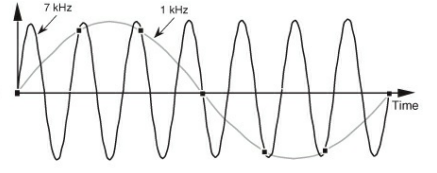
\includegraphics[width=0.75\linewidth]{Figures/aliasing.png}
                \caption[Aliasing example]{Example of aliasing, sampling analoge frequencies of 7 kHz and 1 kHz. Source:\cite{understanding_dsp}, Chapter 2}
                \label{fig:aliasing}
            \end{figure}

        \begin{equation}
        \label{eq:aliasing_x_n}
            x(n) = \sin{(2\pi f_0 n t_s)} = \sin{(2\pi(f_0 + kf_s) n t_s)} 
        \end{equation}
\newpage
        \subsubsection{The Half-Nyquist}
            The Half-Nyquist, is the frequency interval of Equation~\ref{eq:half_nyquist}, where after sampling the frequencies outside of this interval are aliased into this frequency band. This is useful, because it defines the unique frequency range that can be represented by the sampled signal, without ambiguity (\cite{understanding_dsp}, Chapter 2). 

    \begin{equation}
        \label{eq:half_nyquist}
        -\frac{fs}{2} < f <\frac{fs}{2}
    \end{equation}

    
    \begin{figure}[h]
        \centering
        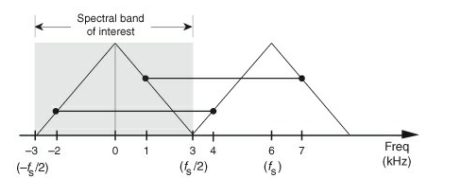
\includegraphics[width=0.75\linewidth]{Figures/half_nyquist.png}
        \caption[Nyquist example]{Example of Half Nyquist. Source:\cite{understanding_dsp}, Chapter 2.}
        \label{fig:half_nyquist}
    \end{figure}
   
    \subsection{Pulse Density Modulation (PDM)}
        \label{sec:PDM}

    % What is it? ok 
    % How does it represent the sound? Bit density? ok 
    % Use that as the reference:
    % - https://www.st.com/resource/en/application_note/an5027-interfacing-pdm-digital-microphones-using-stm32-mcus-and-mpus-stmicroelectronics.pdf
    % -https://users.ece.utexas.edu/~bevans/courses/rtdsp/lectures/10_Data_Conversion/AP_Understanding_PDM_Digital_Audio.pdf

    % REMEMBER TO MENTION THAT PDM IS EQUIVALENT TO THE SIGNAL FROM SIGMA_DELTA ADC !
    Pulse Density Modulation (PDM) is a method for representing the analoge sound signal as a high frequency bitstream of binary one and zero. The amplitude of the analoge signal is represented by increasing or decreasing the period of when the bianry '1' and '0' are present. If the density of '1' is high, the amplitude of the signal is positive, while the high density of '0' corresponds to the negative amplitude of the signal. Increase in the number of binary numbers may also correspond to the rate of change of the ampitude, signaling the rising or falling of the amplitude over time as shown in Fogure~\ref{fig:pdmvssinewave} (\cite{st_an5027_2019}, p.12). 

    \newpage
    \begin{figure}[h]
        \centering
        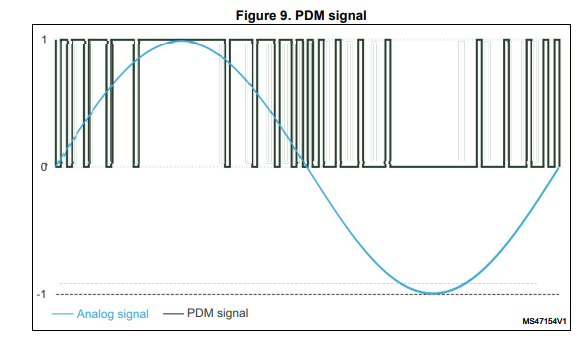
\includegraphics[width=0.75\linewidth]{Figures/PDM vs Sinewave from AN5027.png}
        \caption[Analoge and PDM signals]{Represntation of the analoge signal and it's corresponding PDM signal. Source:(\cite{st_an5027_2019}, p.12)}
        \label{fig:pdmvssinewave}
    \end{figure}

 % What is needed to "understand" the signal in this form? ok
 % The need of filtering and decimation of the signal? ok
    
    The digital microphones sending the PDM signal are able to send up to 3.25 Mbit/s of data, according to manual (\cite{st_mp34dt06j_2021}, Table 2, p.3), which can be unnececary overwhealming, and some of the operations, such as signal processing requires the use of PCM values. Thus the PDM to PCM conversion has to be applied (\cite{kite2012pdm}).


    \subsection{Pulse Code Modulation (PCM)}
    \label{sec:PCM}
    % What is a PCM signal?

    % https://books.google.no/books?hl=no&lr=&id=8l_o6kI3760C&oi=fnd&pg=PR13&dq=pulse+density+modulation+and+pulse+code+modulation&ots=nqlhYDIJRi&sig=ygAAOwsanJ5PmlTM_uisdlnUuIc&redir_esc=y&safe=strict#v=onepage&q=pulse%20density%20modulation%20and%20pulse%20code%20modulation&f=false

    %https://research.ebsco.com/c/qhbpyc/search/details/6evwwwovxr?request-context=plink&db=nlebk
    % https://users.ece.utexas.edu/~bevans/courses/rtdsp/lectures/10_Data_Conversion/AP_Understanding_PDM_Digital_Audio.pdf

    Pulse Code Modulation (PCM) is a method of representing the audio signal digitally, similarly to the PDM, with the main difference of storing the signal with more then just one bit. The method has two main properties needed to properly store the measured signal. It is the sampling rate, which dictates how many discrete samples per second are taken from the audio signal ,effectively limiting the bandwidth of the signal. The next property is the bit depth, or the wordlength, which determines the number of bits which represent each sample of the signal (\cite{st_an5027_2019}, p.12). Additionally the last property is also used to determine the theoretical Signal-to-Noise-Ratio (SNR) of each sample, based on the following Equation~\ref{eq:SNRWordLength} taken from (\cite{kite2012pdm}, p.4). The further explenation of SNR, can be found in the following Section~\ref{Sec:SNR} and the PCM is visualized in the following Figure~\ref{fig:PCM}.  

    \begin{equation}
        SNR = 6.02*N + 1.75
        \label{eq:SNRWordLength}
    \end{equation}

    \begin{figure}[h]
        \centering
        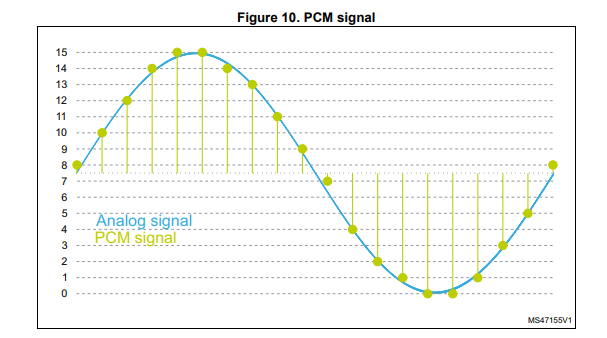
\includegraphics[width=0.75\linewidth]{PCM.png}
        \caption[Analoge and PCM signals]{Represntation of the analoge signal and it's corresponding PCM signal. Source:(\cite{st_an5027_2019}, p.13)}
        \label{fig:PCM}
    \end{figure}
    
\newpage
    
    \subsection{PDM to PCM Conversion}
    \label{sec:PDMtoPCM}

     To correctly convert the PDM into PCM signal, the sample rate of PDM has to be reduced, by a "decimation" factor, (where the dacimtation is the name of the reduction process) to achive the desired sampling frequency of the PCM signal. Decimation also works as the filtering procedure, where the samples outside of the passbond, are removed to reduce the influence of the noise onto the signal (\cite{kite2012pdm}, p.8 and \cite{st_an5027_2019}, p.13).

    
    % https://books.google.no/books?hl=no&lr=&id=8l_o6kI3760C&oi=fnd&pg=PR13&dq=pulse+density+modulation+and+pulse+code+modulation&ots=nqlhYDIJRi&sig=ygAAOwsanJ5PmlTM_uisdlnUuIc&redir_esc=y&safe=strict#v=onepage&q=pulse%20density%20modulation%20and%20pulse%20code%20modulation&f=false

    %https://research.ebsco.com/c/qhbpyc/search/details/6evwwwovxr?request-context=plink&db=nlebk
    % https://users.ece.utexas.edu/~bevans/courses/rtdsp/lectures/10_Data_Conversion/AP_Understanding_PDM_Digital_Audio.pdf
    
    % Low-pass filtering? ok
    % Decimation? ok
    % how does it reconstruct the amplitude?
    % Add nyquist (maybe)?

    

    \subsection{Signal-to-Noise-Ratio (SNR)}
    
    \label{Sec:SNR}

    It is assumed that most of the audio signals measured by the microphones contain a certain level of noise. To quantify the level of noise relative to the actual signal,
    the Signal-to-Noise-Ratio (SNR) is used.
    
    The SNR is defined as the ratio of power between the noise-free signal, and the total measured noise. The value is represented in dB, and can be either negative which represents the stronger noise power over the desired signal or the opposite with the positive value.
    SNR can be estimated using the following Formula~\ref{eq:SNR}, which was taken from (\cite{understanding_dsp}, Appendix D, Sections D5-D5.1).
    
    \begin{equation}
        \label{eq:SNR}
        SNR_{dB} = 10 \log_{10}(\dfrac{P_{signal}}{P_{noise}})
    \end{equation}

\section{Frequency-domain analysis}
This section presents the theoretical background for the frequency-domain analysis methods used in the project.

\subsection{Frequency Transform}
    The Frequnecy Transform (FT) is a method of representing a continous time domain signal, as a continous and infinite frequency domain signal, by using the following Equation~\ref{eq:FT} taken from (\cite{understanding_dsp}, p.74). The frequency domain representation provides the inforamtion of which frequency components are present in the signal, and how strong they are,

    \begin{equation}
    \label{eq:FT}
    X(f) = \int_{-\infty}^{+\infty} x(t) e^{-j 2\pi f t} \, dt
    \end{equation}

    \subsubsection{Discrete Fourier Transform}
    \label{sec:FFT}
    % explain general framing
    % explain general windowing 
    % explain spectral leakage
    Discrete Fourier Transform (DFT) represent a finite discrete-time signal as a discrete signal in the frequency domain. It is a variation of the Fourier Transform (FT) that can be easly understood by the modern machines due to the discrete nature of the output signal, that holds the spectral information such as the signal amplitude and the signal's phase. To apply the DFT, it has to be provided the discrete input signal, which has to be discretized, if originally being obtaing in the analoge form. The DFT represented by the following Equation~\ref{eq:DFT}, taken from (\cite{understanding_dsp}, p.75), uses the provided samples, to convert the signal into equally spaced frequency points which holds the previously mentioned spectral inormation. The frequncy points depend on frequency sampling (fs) and the number of samples (N). An increase of both of the values, may result in more detailed output signal, as the higher number of (N) provides the DFT with finer resolution, and the higher (fs) provides a larger frequency range (\cite{understanding_dsp}, p.74-76). On the other hand the increase of (N) may result in higher compuatational demand, due to the direct dependence of the transform on ($N^2$) as proved by Equation~\ref{eq:O_DFT}, inspired by (\cite{oppenheim_dft_lecture}, p.6) and (\cite{moler_eddins_fft}).

    \begin{equation}
    \label{eq:DFT}
    % taken from understanding..... 3-2 p74/75
        X(m) = \sum_{n=0}^{N-1} x(n) e^{-j 2\pi mn / N}
    \end{equation}

    \begin{equation}
        \label{eq:O_DFT}
        DFT_{computational \ complexity } = O(N^2)
    \end{equation}
    \subsubsection{Fast Fourier Transfor}
    \label{sec:FFT}
    To solve the problem, of DFT puting a high computational demand on the computer systems, the Fast Fourier Transform (FFT) was developed by John Cooley and John Tukey in 1965 (\cite{understanding_dsp}, p.138).
    The FFT and specifically radix-2 FFT is "a very effieicent alogrithm" (\cite{understanding_dsp}, p.138) that simplifies the DFT by eliminating the need of computing the redundant values, by "exploiting symmetry and periodicity properties of the complex exponential sequences" (\cite{oppenheim_dft_lecture}.p6).
    Hence the algorithm allows to conduct DFT of many samples in much reduced time, as the need for computation is greatly reduced as proved in Equation~\ref{eq:O_FFT}, taken from (\cite{understanding_dsp}, p.139). The superiority of FFT over DFT in terms of the reduced number of computations can be visualized by the Figure~\ref{fig:DFTvsFFT}]. However according to \cite{goyal2015condition}, p.8, the FFT has restricitions which doesn't allow it to depict spectral changes of the signal over time, which forces the implemnetation of Short-time Fourier Transform (STFT) which is used to extract the content of the non-stationary signal, such as sound produced by a moving drone. The STFT is conducted by framing the signal into short windows as that assumes stationary of the signal and then by applying the FFT on each window (\cite{goyal2015condition}, p.8).     

    \begin{figure}[h]
        \centering
        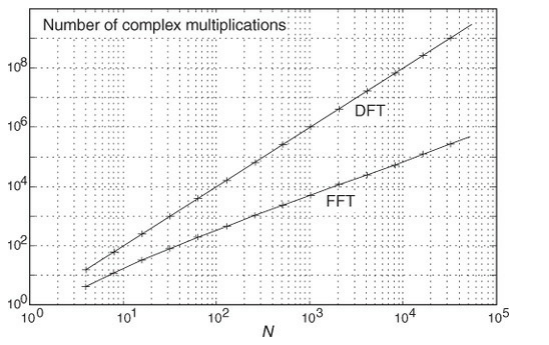
\includegraphics[width=0.5\linewidth]{DFTvsFFT.png}
        \caption[Number of complex multipliactions]{Number of complex mulitplications as a function of N, for FFT and DFT, Source:(\cite{understanding_dsp}, p.139)}
        \label{fig:DFTvsFFT}
    \end{figure}

    \begin{equation}
    \label{eq:O_FFT}
        FFT_{computational \ complexity} =O(\frac{N}{2}\log_2N)
    \end{equation}
\newpage
    \subsubsection{IDFT}
    \label{sec:IFFT}

    Inverse Discrete Fourier Transfrm (IDFT) is a method of converting the frequency domain signal into the time domain. The method may be applied, when the signal has been filtered, or modified in the frequency domain, but it's final form has to be represented in the time domain. The method is applied by utilizing the Equation~\ref{eq:IDFT}, taken from (\cite{understanding_dsp}, p.92) 

    \begin{equation}
    \label{eq:IDFT}
    x(n) = \frac{1}{N} \sum_{m=0}^{N-1} X(m) e^{j 2\pi m n / N}
\end{equation}

    \subsection{Windowing}
    \label{sec:Windowing}
    Windowing is a way of reducing the results of the spectral leakge, which occurs when there exists frequency components inside of the measured signal, that are not exactly represented by the fundamental frequency Equation~\ref{eq:f_fund}), and by it's integer multiplies (commonly known as the analysis frequencies). The analysis frequency can be found by utilizing Equation~\ref{eq:f_analysis} taken from (\cite{understanding_dsp}, p.92). The result of the spectral leakge may be described as a leakge of energy, that spreads into multiple frequency bins, outputted by the DFT and is visualized in the Figure~\ref{fig:Leakages}. The spectral leakge, is a persistent issue, that effects can only be minimized and not fully adressed (\cite{understanding_dsp}, p.92-95). One of the methods used to minimize the issue, is the application of windowing functions, such as Hanning or Hamming functions, that froces the amplitude of the finite signal at the begining and at the end of the signal segment to move towards zero, as seen in Figure~\ref{fig:windows}. As the DFT can only be applied on the finite time signals, the signal is by default windowed using the rectangle function, which causes the amplitude of the signal to sharply move from 0 to 1. That sharp move is the reason for the existance of the sidelobes in DFT magnnitude output, which also causes the spectral leakage as visualized in Figure~\ref{fig:sidelobes_windowing_effects}. The figure also proves that Hanning and Hamming would be the most suitable for the project application, due to their reduction of the sidelobes, which also reduces the leakage of energy into neighboring bins (\cite{understanding_dsp}, p.99-102).

\begin{equation}
\label{eq:f_fund}
    f_{fundamental} = \frac{fs}{N}
\end{equation}

\begin{equation}
\label{eq:f_analysis}
    f_{\text{analysis}}(m) = \frac{m f_s}{N}, \quad \text{where } m = 0,1,2,\ldots,N-1
\end{equation}
    
\begin{figure}[H]
    \centering
    
    \begin{subfigure}{0.45\linewidth}
        \centering
        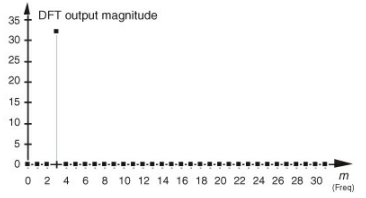
\includegraphics[width=\linewidth]{Figures/No_leakage.png}
        \caption{Magnitude of the DFT without the leakge}
    \end{subfigure}
    \hfill
    \begin{subfigure}{0.45\linewidth}
        \centering
    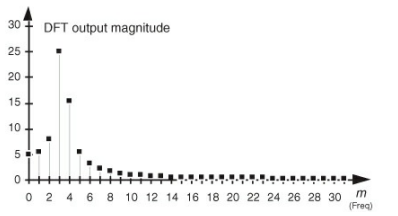
\includegraphics[width=\linewidth]{Figures/leakage_present.png}
        \caption{Magnitude of the DFT with leakge present}
    \end{subfigure}
\caption[Response without the leakage vs with the leakage]{Comparison between the DFT magnitude without the leakage and with the leakge present. Source: \cite{understanding_dsp}, p.93-94}
    \label{fig:Leakages}
\end{figure}


\begin{figure}[H]
    \centering
    
    \begin{subfigure}{0.45\linewidth}
        \centering
        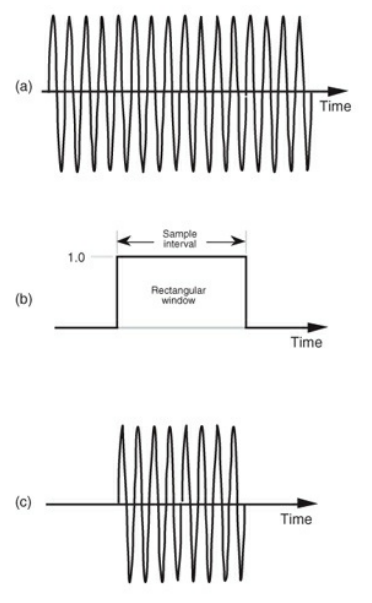
\includegraphics[width=\linewidth]{rectangle.png}
        \caption{Rectangular window}
    \end{subfigure}
    \hfill
    \begin{subfigure}{0.45\linewidth}
        \centering
        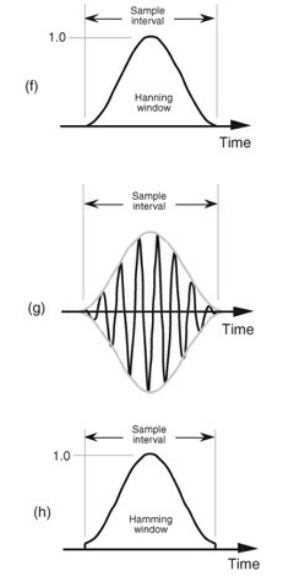
\includegraphics[width=\linewidth]{Hanning.png}
        \caption{Hanning window}
    \end{subfigure}
    
    \caption[Rectangular vs hanning window]{Comparison of rectangular and Hanning window functions and the result of applying them on the infinite time signal. Source: \cite{understanding_dsp}, p.100}
    \label{fig:windows}
\end{figure}

\begin{figure} [H]
    \centering
    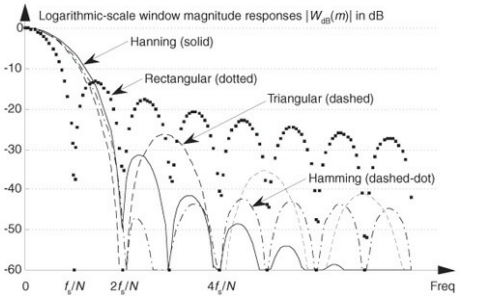
\includegraphics[width=0.75\linewidth]{Figures/sidelobes_windowing.png}
    \caption[Windowing effects]{Effects of windowing functions on side lobe creation. Source: \cite{understanding_dsp}, p.102}
    \label{fig:sidelobes_windowing_effects}
\end{figure}

\subsection{Sinc function as a digital filter}
\label{sec:sinc_filter}
The sinc function can be expressed as in the following Equation~\ref{eq:sinc}, taken from \cite{understanding_dsp}, Section 3.8, though a bit modified to represent the continous function. The function represents the behaviour of the moving-average filter, where the input data is averaged over the set number of previous samples (\cite{stm_an4990_dfsdm}, Section 3) as in the following Equation~\ref{eq:moving_average} from (\cite{understanding_dsp}, Section 10.14.1). The filter can be designed as described in Figure~\ref{fig:moving_avg_schematic}, however the D, has be changed with FOSR in the schematic, but they still represent the same number. Additionaly the digtal signal that has been filtered, can be processed again, if the higher order of the sinc function is applied. However the additional processing of the signal, in addition to attenuating the unwanted frequencies, can also attenuate the desired frequencies as in the concept figures: Figure~\ref{fig:comparison_of_signals_with_sinc} and Figure~\ref{fig:mag_response_sinc}, where the aplication of the 3rd-order sinc reduces the original signals magnitude to around 37\% of the original value, despite the reduction of the side lobes.


\begin{equation}
    \label{eq:sinc}
    sinc(x) = \frac{\sin(\pi x)}{\pi x}
\end{equation}

\begin{equation}
    \label{eq:moving_average}
    y(n) = \frac{1}{D}[x(n) + x(n-1) + ... + x(n - D + 1)] = \frac{1}{D}\sum^{D-1}_{k = 0}x(n-k)
\end{equation}

\begin{figure}[h]
    \centering
    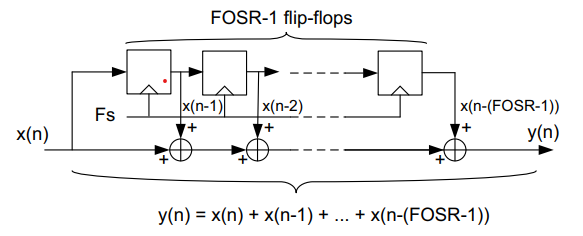
\includegraphics[width=1\linewidth]{Figures/basic_moving_avg_schematic.png}
    \caption[Moving average example]{A basic schematic for a moving average filter. Source: \cite{stm_an4990_dfsdm}, Figure.10}
    \label{fig:moving_avg_schematic}
\end{figure}

\newpage

\begin{figure}[h]
    \centering
    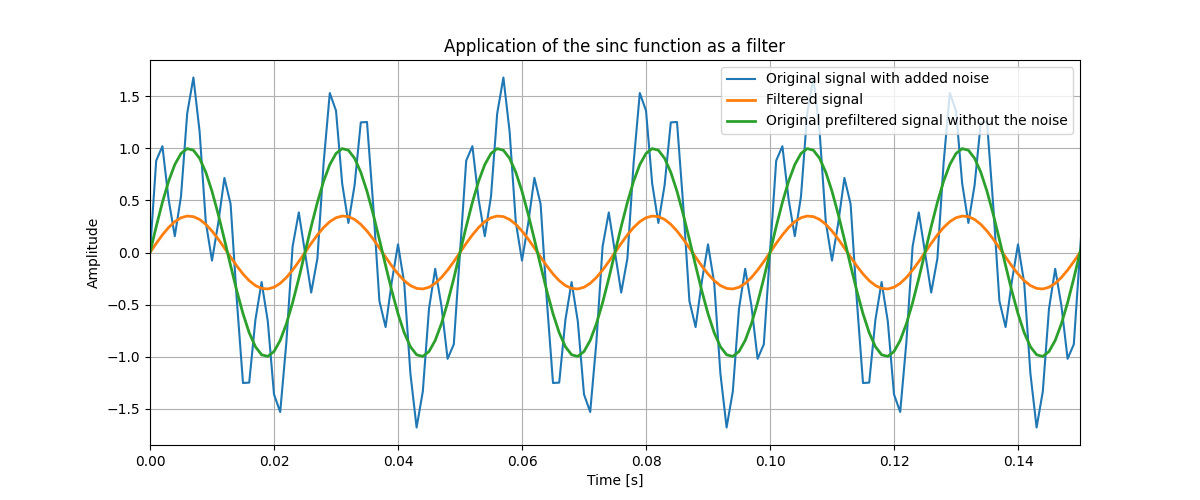
\includegraphics[width=1\linewidth]{filtering of a signal with sinc.png}
    \caption[Original vs filtered signal example]{Comparison of the original signal ($\sin{(2\pi 40t)})$, with added noise of $0.7\sin{(2\pi 180t)}$, and the final signal filtered with the sinc function and the sampling frequency of 1000. }
    \label{fig:comparison_of_signals_with_sinc}
\end{figure}

%wanted = np.sin(2 * np.pi * f_wanted * t)
%unwanted = 0.7 * np.sin(2 * np.pi * f_unwanted * t)

\begin{figure} [h]
    \centering
    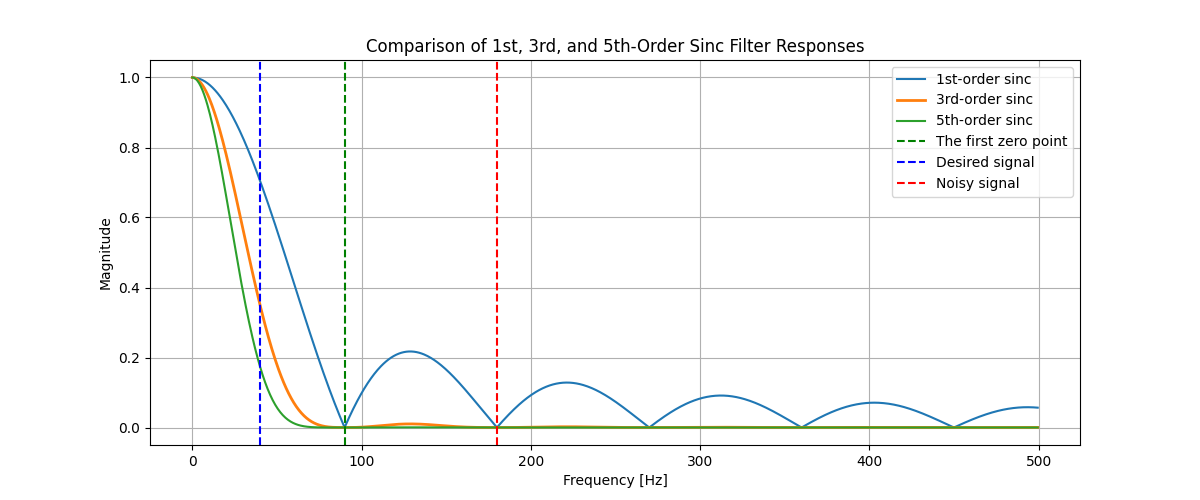
\includegraphics[width=1\linewidth]{Figures/sinc function mag responses.png}
    \caption[Example responses of the sinc based filters]{Magnitude responses of sinc based filters of different order}
    \label{fig:mag_response_sinc}
\end{figure}


\newpage

\section{Direction of arrival (DOA) estimation}
   The Direction of arrival (DOA) describes the direction from which the acoustic signal reaches the microphones. The DOA can be estimated by measuring the Time difference of arrival (TDOA) between microphone pairs and relating theses delays to the physical geometry of the microphone array, and the sound speed as expressed in Equation~\ref{eq:tau}. In this relation, \textbf{d} represents the distance between the microphone in the pair, \textbf{c} stands for the sound speed and \textbf{$\theta$} denotes the angle of arrival of the sound source relative to the normal vector of the microphone pair (\cite{blandin2012multisource}). The relation is valid under the far-field assumption, which assumes that the distance between the sound source and the microphone array is larger then the distance between the microphones.   

    \begin{equation}
        \label{eq:tau}
        \tau = \frac{d}{c}\cos(\theta)
    \end{equation}

    \subsection{Time Difference of Arrival (TDOA)}
    \label{sec:TDOA}
    % Propagation delay
    % Geometry
    % Relationship between the distance and delay and angle 
    % Limitation caused by tge mic spacing
    % Max phisically possible lag
    % Near filed and far filed assumptions
    The Time Difference of Arrival (TDOA) represents the time difference in arrival time of the acoustic signal between a pair of spatially separated microphones. Effectively representing which microphone in the pair, was first to receive the acoustic signal. To achieve that, the project uses the generalized cross-correlation (GCC) which estimates the TDOA of a microphone pair, and later uses the microphone geometry to estimate the direction of arrival (DOA) of the signal source (\cite{kwon2010gccphat}, \cite{blandin2012multisource} and \cite{kang2016prefiltering}). 


    \subsection{Generalized Cross-Correlation with PHAT weighting (GCC-PHAT)}
    \label{sec:gcc}
    The GCC represents the degree of correlation between the signals from a microphone pair over different time lags. The correlation is computed in frequency domain by finding the cross-power spectrum (CPS) of the microphone pair. In GCC-PHAT, the CPS is adjusted by PHAT weighting with additional factor $\beta$, which reduces the influence of large-amplitude frequency components and makes the TDOA estimation more dependent on the phase difference between the microphone signals. %This may improve the robustness of the delay estimation, although noisy frequency components can still affect the result 
    (\cite{kang2016prefiltering} and \cite{kwon2010gccphat}).
    
    \subsubsection{Cross-power spectrum (cps)}
    \label{sec:cps}
    The Cross-power spectrum between the microphones, is found by multiplying the frequency-domain signal from one microphone, with the conjugate of the signal from the second microphone as in the following Equation~\ref{eq:gcc}. % from \cite{kang2016prefiltering}.
    The output of the CPS represents the relation between the microphone signals for each frequency bin $k$, which includes the magnitude relationship and the phase difference caused by the time delay between the microphones (\cite{kang2016prefiltering}).

    \begin{equation}
    \label{eq:gcc}
        G(k) = X_1(k)X_2^*(k)
    \end{equation}


    \subsubsection{PHAT weighting}
    \label{sec:PHatW}
    PHAT weighting 
    is used to reduce the influence of the high amplitude frequencies, that may shadow other, weaker frequency components, by normalizing the amplitudes of their CPS values as in the Equation~\ref{eq:phat}. Additionally the PHAT can be adjusted by the $\beta$ weight, that may vary from 0 to 1, based on the SNR value, or any other application-specific criteria (\cite{kang2016prefiltering}).       

    \begin{equation}
        \label{eq:phat}
        \Psi^\beta (k) = \frac{1}{|G(k)|^\beta}
    \end{equation}
    
    \subsubsection{Delay estimation from the GCC function}
    \label{sec:delay_estimation_from_gcc}
        The time differnce can be estimated by finding the lag that is maximizing the GCC-PHAT output as in the following Equation~\ref{eq:r_l} %from \cite{kang2016prefiltering}
        , where the GCC output is weighted by the PHAT function and then transformed back to the time-domain (\cite{kang2016prefiltering}).

    \begin{equation}
        \label{eq:r_l}
        \max r(l) = F^{-1}(\Psi^{\beta}(k)G(k))
    \end{equation}

    
\section{Feature extraction}
This section presents the theoretical background for the feature extraction methods used in this project.

    \subsection{Mel scale}
    \label{sec:MEL}

    The Mel scale is a frequency scale that approximates how humans perceive pitch. In MFCC feature extraction, the power spectrum \(P(f)\) is wraped from the Hertz frequency axis to the Mel-frequency axis as \(P(M)\) in order to approximately reflect human ear percetion. A frequency \textbf{f} in Hertz can be converted to the mel scale as in the Equation~\ref{eq:mel} (\cite{zheng2001mfcc}).


    \begin{equation}
        \label{eq:mel}
        M(f) = 2595\log_{10}(1+\frac{f}{700})
    \end{equation}

    \subsection{Mel-frequency cepstral coefficients (MFCC) }
    \label{sec:MFCC}
    The MFCC is a feature extraction method used to represent the short-term spectral characteristics of an acoustic signal. The information about spectral characteristics is stored in the MFC coefficients, which number can vary, and can either increase or decrease the computational time needed to extract the features. To extract the MFCC features, the extraction algorithm can follow the following pipeline Figure~\ref{fig:mfcc_pipeline} (\cite{singh2014mfcc}).

    \begin{figure}[h]
        \centering
        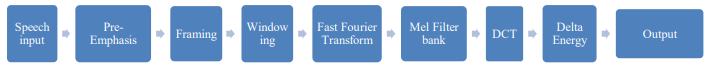
\includegraphics[width=1\linewidth]{Figures/MFCC_pipeline.png}
        \caption[Example pipeline for MFCC]{Example pipeline for the extraction of the MFCC features. Source: \cite{singh2014mfcc}}
        \label{fig:mfcc_pipeline}
    \end{figure}

    \subsubsection{Pre-emphasis}
    \label{sec:pre_emp}
    The pre-emphesis stage of the MFCC extraction is used to emphasize the higher-frequency components present in the signal before the further feature extraction. This increases the energy levels of the high-frequency components present in the measured signal (\cite{singh2014mfcc} and \cite{librosaPreemphasis}). An example of how the pre-emphesis can change the signals energy content can be seen in Figure~\ref{fig:pre-emphesis example}.

    \begin{figure}[h]
        \centering
        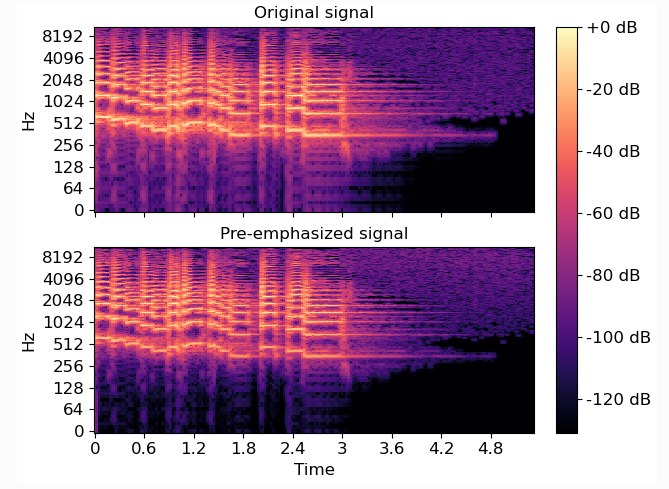
\includegraphics[width=0.5\linewidth]{Figures/example of pre-emphesis.png}
        \caption[Pre-emphesis example]{An example of how the pre-emphesis can change the energy content of the signal. Source:\cite{librosaPreemphasis}}
        \label{fig:pre-emphesis example}
    \end{figure}
    
    \subsubsection{Framing}
    Framing is used to divide the signal into short-duration frames because of the time-varying nature of acoustic signals. Within a short frame such as 25 ms, the signal can be treated as approximately stationary, since the frame contains data from only a short time interval (\cite{singh2014mfcc}).

    
    \subsubsection{Mel filter bank (MLB)}
    The MLB is used to convert the signal's magnitude response in the frequency domain to the mel-scale based response. This is achived by multiplying the magnitude response of the signal with a set of K-number band-pass filters of triangular or rectangular shape wich may, or may not overlap with each other. The filter forms can be as in the Figure~\ref{fig:band_pass_filters} (\cite{singh2014mfcc} and \cite{zheng2001mfcc}).


    \begin{figure} [h]
        \centering
        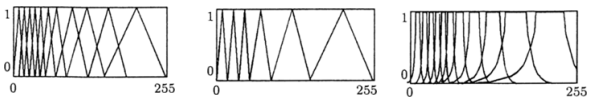
\includegraphics[width=1\linewidth]{Figures/mel_bank_filters.png}
        \caption[Band-pass filter]{The Band-pass filters used in the process of extraction the MFCC. Source: \cite{zheng2001mfcc}}
        \label{fig:band_pass_filters}
    \end{figure}

    % Should i even write about that, if I have no use to that in the method? However i do use the default type 2 DCT, when using MFCC from librosa 
    %\subsubsection{Discrete Cosine Transform (DCT)}
    %The DCT 

    \subsection{Delta and Delta-Delta features}
    \label{sec:deltadelta}
    The delta and delta-delta represents the rate of change, and acceleration of the cepstrum represented by the MFCC. The delta can be found by taking the first-order time derivative and the delta-delta by the second-order time derivative (\cite{singh2014mfcc}).
    

\section{ML classification}
\subsection{YOLO Object Detection}

YOLO (You Only Look Once) is a real-time single-stage object detection 
model based on Convolutional Neural Networks (CNNs). Unlike two-stage 
detectors such as Faster R-CNN, which require separate region proposal 
and classification passes, YOLO divides the input image into a grid and 
performs both object localization and classification in a single forward 
pass, achieving significantly faster inference speeds (\cite{redmon2016yolo}). 
Where R-CNN takes around 47 seconds to process a single image due to 
classifying approximately 2000 region proposals, YOLO processes the entire 
image in one shot, making it far more suitable for time-sensitive 
applications (\cite{vijayakumar2024yolo}). Since its introduction in 2015, 
the model has undergone continuous architectural refinement, with each 
version addressing specific limitations of its predecessor 
(\cite{vijayakumar2024yolo, sapkota2025ultralytics}).

\vspace{1em}

Key milestones in this evolution include YOLOv2, which introduced anchor 
boxes and batch normalization (\cite{vijayakumar2024yolo}); YOLOv3, which 
deepened the backbone to Darknet-53 and added multi-scale feature 
prediction through a Feature Pyramid Network (FPN) (\cite{vijayakumar2024yolo}); 
and YOLOv4, which incorporated CSPDarknet-53, a Path Aggregation Network 
(PANet) neck, and the CIoU loss function (\cite{vijayakumar2024yolo}). 
YOLOv5 marked a decisive shift to a fully PyTorch-native implementation, 
introducing five modular depth- and width-scaled variants and a unified 
training and export toolchain (\cite{vijayakumar2024yolo, sapkota2025ultralytics}).


\subsection{YOLOv8 Architecture}

YOLOv8, released by Ultralytics in January 2023, follows the standard 
three-part structure of backbone, neck, and head that became established 
from YOLOv3 onwards (\cite{vijayakumar2024yolo}), and introduces targeted 
improvements at each stage (\cite{vijayakumar2024yolo, sapkota2025ultralytics}).

\vspace{1em}

The \textbf{backbone} replaces earlier C3 modules with a new C2f module 
--- a Cross Stage Partial structure incorporating two convolutional 
operations and a bottleneck --- which maintains receptive-field richness 
while reducing parameter overhead (\cite{sapkota2025ultralytics}). A Spatial 
Pyramid Pooling Fast (SPPF) layer follows the backbone to aggregate 
context across multiple spatial scales (\cite{sapkota2025ultralytics}). The 
\textbf{neck} uses a PANet-style structure to combine top-down and 
bottom-up pathways, ensuring that both high-level semantic information and 
fine-grained spatial detail flow into the head (\cite{vijayakumar2024yolo}).

\vspace{1em}

The most significant change in YOLOv8 is the fully \textbf{decoupled 
detection head}, which separates the classification and bounding box 
regression branches into two independent streams (\cite{sapkota2025ultralytics}). 
This mitigates gradient interference between the two objectives and 
improves convergence (\cite{sapkota2025ultralytics}). Complementing this, 
YOLOv8 adopts a fully \textbf{anchor-free} design, directly predicting 
normalized bounding box parameters for candidate points on the feature 
map, removing the need for anchor clustering and improving generalization 
across datasets with differing object aspect-ratio statistics 
(\cite{vijayakumar2024yolo, sapkota2025ultralytics}). For bounding box 
regression, YOLOv8 uses the CIoU loss function, and binary cross-entropy 
for classification (\cite{vijayakumar2024yolo}). Following inference, 
Non-Maximum Suppression (NMS) is applied to suppress redundant overlapping 
detections, retaining only the highest-confidence bounding box for each 
object (\cite{vijayakumar2024yolo}).

\vspace{1em}

YOLOv8 is offered in five scaled variants --- nano (n), small (s), 
medium (m), large (l), and extra-large (x) --- which differ in network 
depth and width (\cite{sapkota2025ultralytics}). This thesis uses 
\textbf{YOLOv8n}, the nano variant, which has approximately 3.2 million 
parameters and 8.7 billion FLOPs (\cite{sapkota2025ultralytics}). On the 
MS COCO validation set at 640$\times$640 pixel input resolution, YOLOv8n 
achieves a mean Average Precision (mAP@0.50:0.95) of approximately 37.3\%, 
with a CPU latency of around 80.4\,ms per image (ONNX) and under 1\,ms 
on an NVIDIA T4 GPU (TensorRT) (\cite{sapkota2025ultralytics}).


\subsection{Performance Metrics}

Object detection performance is primarily evaluated using \textbf{Intersection 
over Union (IoU)} and \textbf{mean Average Precision (mAP)} 
(\cite{vijayakumar2024yolo}). IoU measures the spatial overlap between a 
predicted bounding box and the ground-truth box, calculated as the ratio 
of their intersection to their union area, ranging from 0 to 1 
(\cite{vijayakumar2024yolo}). A detection is considered correct only when 
its IoU with the matched ground truth exceeds a set threshold, most 
commonly 0.5 (\cite{vijayakumar2024yolo, sapkota2025ultralytics}).

\vspace{1em}

Precision measures the proportion of predicted detections that are 
correct (TP / (TP + FP)), while Recall measures the proportion of actual 
objects that are successfully detected (TP / (TP + FN)) 
(\cite{vijayakumar2024yolo}). Average Precision (AP) is computed as the 
area under the precision--recall curve for a single class, and mAP 
averages this over all classes (\cite{vijayakumar2024yolo}). YOLO models 
use mAP as the primary metric in preference to the F1 score, as the 
F1 score can be heavily skewed toward majority classes in datasets with 
class imbalance, making it unreliable for evaluating performance on 
minority classes (\cite{vijayakumar2024yolo}). The stricter COCO-style 
evaluation reports mAP@0.50:0.95, averaging AP over ten IoU thresholds 
from 0.50 to 0.95 in steps of 0.05, penalizing imprecise localization 
more heavily than the older Pascal VOC standard (\cite{sapkota2025ultralytics}).

\subsection{Sound classification}
\subsubsection{Convolutional Neural Network}
A Convolutional Neural Network(CNN) is a deep-learning architecture inspired by human pattern recognition. CNNs consist of an input layer, one or more hidden layers, and an output layer, through which they learn to recognise patterns in visual data. The input layer performs pre-processing(e.g., rescaling, normalisation) to bring each image into a standardised representation for further computation. The Hidden part of the model may contain several layer types, including convolutional layers, pooling layers, and fully‑connected layers. Among these the convolutional layer is key: it applies a set of learnable filters to the input, extracting local features and producing a feature map for each filter. Finally the output layer combines the information from the hidden layers into class-probability estimates.(\cite[Chapter 14]{geron2019handson})
\subsubsection{Decision tree}
Decision‑tree learning is a supervised‑learning algorithm that maps a set of input variables onto a target variable. Two main variants exist: classification trees, which predict a categorical class label, and regression trees, which predict a continuous outcome. In the context of this paper, only the classification variant is relevant, whereby the model assigns each input value to one of the predefined classes.(\cite[Chapter 6]{geron2019handson})
        
\section{Hardware}
    This section provides a brief and general description of the hardware present in the system. 
        \subsection{Digital MEMS microphones}
        % WORK IN PROGRESS
        The digital mems microphones, as seen in the example schematic Figure~\ref{fig:mems_block}, are consturated in such a way, that they can convert the acoustic signal (which is in the analog form) into the digital PDM format,easily readable by the peripheral at the MCU.
        The data send from the microphones is controlled by the frequency of the \textbf{CLK} input, which typically is provided a High/Low signal at the frequency between 1 Mhz to 3 Mhz by the connected MCU. 
        The microphones can also allow to select at which moment the microphone should send the data, based on the connection to the \textbf{Channel select}, as in Figure~\ref{fig:stereo_mics}.

        \begin{figure}[h]
            \centering
            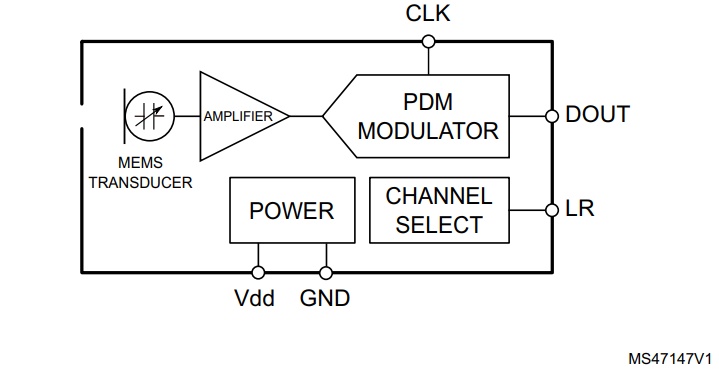
\includegraphics[width=0.75\linewidth]{Figures/mems_mics.png}
            \caption[Example block diagram of mems microphone]{Example block diagram of a mems digital microphone. Source: \cite{st_an5027_2019}}
            \label{fig:mems_block}
        \end{figure}

        \begin{figure}[h]
            \centering
            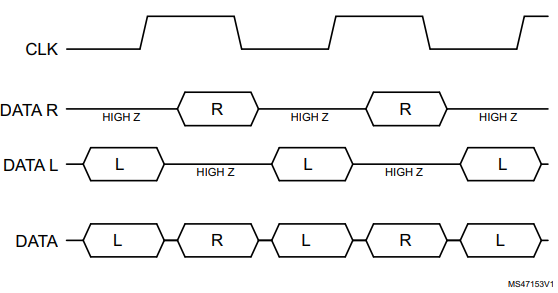
\includegraphics[width=0.75\linewidth]{Figures/stereo_mics_config_data.png}
            \caption[Stereo data pattern]{The Stereo data pattern from the mems microphones. Source: \cite{st_an5027_2019}}
            \label{fig:stereo_mics}
        \end{figure}
    
     % MEMS mics principle:
        % How do they work?
        % What do they need?
    % Analog vs digital mics
        % main differences, but reather short, as only teh digital mics were used.
     % Shared data line and time division
        % Clock signal?
        % Data line?
        % Selection of L/R on Mics?
        % Time multiplexing
    % Use that as the reference:
    % - https://www.st.com/resource/en/application_note/an5027-interfacing-pdm-digital-microphones-using-stm32-mcus-and-mpus-stmicroelectronics.pdf
    % - https://www.st.com/resource/en/data_brief/steval-mic002v1.pdf
    % -https://users.ece.utexas.edu/~bevans/courses/rtdsp/lectures/10_Data_Conversion/AP_Understanding_PDM_Digital_Audio.pdf 
        


        
\section{Communication protocols and peripherals}
    This section provides a theoretical description of the communication protocols present in the system.
    
    \subsection{Digital Filter Sigma-Delta Modulator (DFSDM)}
    The DFSDM is a digital peripheral used for processing and filtering of a 1-bit stream sent by the microphones. The example block diagram of the peripheral can be seen in Figure~\ref{fig:dfsdm_block}.
    The 1-bit stream is produced by a sigma-delta modulator (SDM), which converts the analog acoustic signal into a digital bitstream, as shown in Figure~\ref{fig:sdm}. In the project, the conversion is performed internally by the digital microphones, which outputs the signal as PDM.
    The converted signal is then sent to the microcontroller, where the Digital Filter (DF) applies the digital sinc function of configurable order, as described in Section~\ref{sec:sinc_filter}. The DF can be configured, by changing the order of the sinc function and the oversampling ratio known as FOSR. 
    The output data from the DF, can also be accumulated in the integrator, by changing the value of IOSR, which represents how many samples have to be summed up to return a single sample output. The final output data from the peripheral, is directly determined by the number of the PDM input samples, FOSR and the IOSR number. By changing any of them, the final sample rate will therefore vary. The peripheral to able to correclty process the data signal from the microphones, also has to generate the clock signal, that the microphone will adjust its data signal to (\cite{stm_an4990_dfsdm}).
    
    %The DFSDM uses the digital filter (DF) and the external Sigma-delta modulator (SDM), and as the name implies, filters the digital signal, by applying the sinc-function of freely chosen order, which was already described in more detail in this section [sec:\ref{sec:sinc_filter}. The SDM is responsible for converting the analoge signal into the digital signal that can be later filtered, as in the following schematic [fig:\ref{fig:sdm}]. The project is only using the SDM in such a way, that the microphones are internally converting the analoge acoustic signal into the PDM signal, most probably using the same principle, as described in the Sigma-delta modulation schematic. The converted signal is then sent to the microcontroller in the digital form to be filtered by the peripherial.    

    \begin{figure}[h]
        \centering
        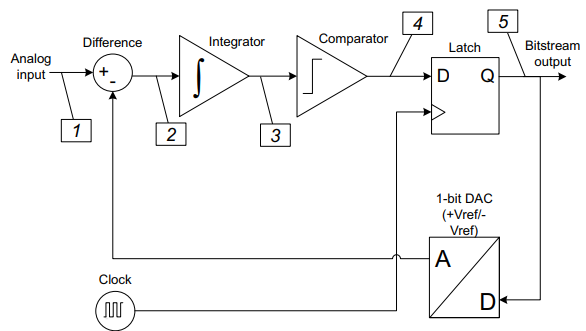
\includegraphics[width=0.5\linewidth]{Figures/sigma_delta_modulation.png}
        \caption[Example of a Sigma-delta modulator schematic]{Sigma-delta modulation schematic. Source: \cite{stm_an4990_dfsdm}}
        \label{fig:sdm}
    \end{figure}

    \begin{figure}[h]
        \centering
        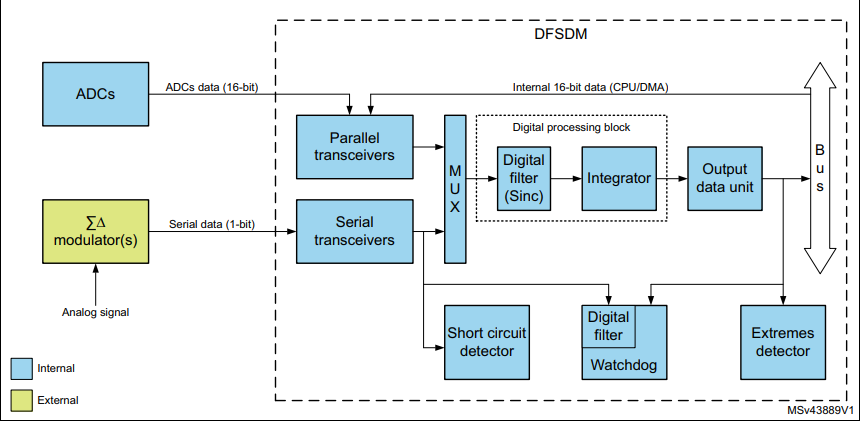
\includegraphics[width=0.5\linewidth]{Figures/dfsdm_internal_block.png}
        \caption[Example of a DFSDM block diagram]{DFSDM block diagram. Source: \cite{stm_an4990_dfsdm}}
        \label{fig:dfsdm_block}
    \end{figure}
    \newpage
    \subsection{Serial Audio Interface (SAI)}
    Tha SAI is an interface that can be used to receive the data signal from the digital microphones. The SAI can operate with its own audio clock generator, or the external timer, which can generate the clock signal for the microphones. The interface can operate with two sub-blocks, which can gather data independently. If the interface is gathering the data only from one microphone per line, the bit content should be as in the Figure~\ref{fig:mono_sai}, where the bits from the microphone are stored in a byte in the memory and accesd through the Direct Memory Acces (DMA). However When gathering the data from two microphones connected to the same line, the bit content will vary as it will be as in the Figure~\ref{fig:stereo_sai}, where each odd bit represent the data from one microphone, and the even one represent the second microphone. The resulting bit-stream from the microhpones is therefore interleaved, and need the additional de-interleaving algorithm to separate the bits from each other. (\cite{st_an5027_2019}).


\begin{figure}[h]
    \centering
    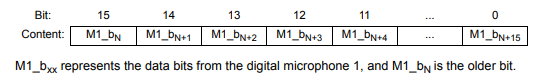
\includegraphics[width=0.75\linewidth]{mono_sai.png}
    \caption[Example of a mono bit configuration for SAI]{Bit configuration for the mono setup of SAI. Source: \cite{st_an5027_2019}}
    \label{fig:mono_sai}
\end{figure}



\begin{figure}[h]
    \centering
    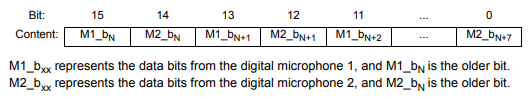
\includegraphics[width=0.75\linewidth]{Figures/stereo_sai.png}
    \caption[Example of a stereo bit configuration for SAI]{Bit configuration for the stereo setup of SAI. Source: \cite{st_an5027_2019}}
    \label{fig:stereo_sai}
\end{figure}
\newpage

    \subsection{USART/UART}
    Universal Synchronus/Asynchronus Receiver Transimter (USART/ UART) are variations of a communitation protocol used in the early stages of the project. The protocol is able to send the data from the transmitter in the asynchronus mode, where the receiver does not share the synchronization clock signal with the transmitter, hence it has to be manually configured before use with the same baud rate as the transmitter. However in the synchronus mode, the receiver and the transmitter both share the data and the clock lines, where the clock line aligns the data signal, without the need of prior data configuration. The frame format of a typical UART protocol is as in Figure~\ref{fig:uart_frame}, which contains the idle High bit, the low start bit , the data bit, the low parity bit and the high stop bit, which add up to 10 bits per second. Based on the following online calculator \cite{lucidar_baud_bytes}, the Bytes per second can be found by using the following Equation~\ref{eq:bytes_per_second_baud}
    where the \textbf{$BR_{bauds}$} represents the baud rate and the \textbf{bits per frame} are in this case equal to 10 bits per second per frame (\cite{stm_uart}, \cite{techtarget_usart} and \cite{laddha2013uart}).


    \begin{figure}[h]
        \centering
        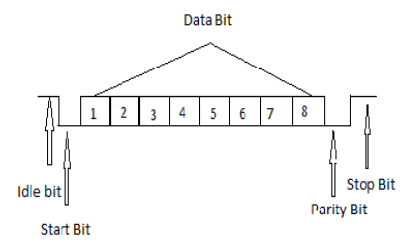
\includegraphics[width=0.5\linewidth]{Figures/uart_bit_map.png}
        \caption[Example of a UART frame format]{The typical UART frame format. Source: \cite{laddha2013uart}}
        \label{fig:uart_frame}
    \end{figure}

    \begin{equation}
        \label{eq:bytes_per_second_baud}
        BR_{gross} = \frac{BR_{bauds}}{bits \space  per \space frame}
    \end{equation}
    
    \subsection{USB}
    The Universal serial bus (USB) is a serial communication standard introduced to standardize the communication between the host and the device, and at the same time provide them with high speed transfer capabilities. The USB devices can be implemented using different device classes, which dictates how the devices will communicate with each other, depending on the devices application and function. The transfer speeds used by the USB 2.0, which was also used in the later stage of the project, can be divided into the following three categories:\\
    \\
    - Low speed (LS) which supports the speed of up to 1.5 Mb/s,\\
    - Full speed (FS) that can transfer the data with the speed of up to 12 Mb/s,\\
    - High speed (HS) which is the fastet one, providing the user with the transfer speed of up to 480 Mb/s.\\
    (\cite{stm_usb}).
    
    
    
    \subsection{MQTT}
    
Message Queue Telemetry Transport (MQTT) is a lightweight publisher/subscriber communication protocol designed for efficient message exchange. In a pub/sub system, publishers send messages to a named topic, which are then received by any clients subscribed to that topic. MQTT brokers act as intermediaries, holding and distributing messages between clients, which can function as both publishers and subscribers simultaneously (\cite{soni2017mqtt}).


    \subsection{UDP}
    
The User Datagram Protocol (UDP) is a connectionless transport protocol that sends
data packets without establishing a dedicated connection or guaranteeing delivery,
ordering, or error correction (\cite{rfc3550}). Unlike TCP, UDP does not retransmit
lost packets, which makes it particularly well suited for real-time video streaming.
In a live video feed, a retransmitted packet arriving late is more disruptive than
a dropped frame, as it introduces latency and stuttering that degrades the viewing
experience (\cite{rfc3550}). For this reason, real-time video applications commonly
rely on UDP as the underlying transport protocol, accepting occasional packet loss
in favour of low and consistent latency.

\subsection{H.264}

H.264, also known as MPEG-4 AVC, is a widely used video compression standard
developed jointly by the ISO/IEC MPEG group and the ITU-T Video Coding Experts
Group. Compared to its predecessor MPEG-2, H.264 achieves perceptually equivalent
video quality at roughly one-third to one-half of the bitrate, making it well suited
for bandwidth-constrained applications such as network video streaming (\cite{1709847}).

H.264 is a block-based hybrid video codec, meaning it reduces redundancy in video
data through a combination of motion compensation and transform coding. Video frames
are divided into $16 \times 16$ pixel macroblocks, which are processed using one of
several frame types: intra-coded (I), predictive (P), or bipredictive (B) frames
(\cite{1709847}).

\subsection{Project Management}
Scrum is an agile project‑management framework designed to coordinate complex, knowledge‑intensive initiatives through iterative and incremental development. Scrum Organizes its workflow into sprints. Sprints are short time periods usually chosen to be one to four weeks. At the end of the sprint a meeting is held to walk through the achieved goals and the goals for the next sprint. There usually also is frequent meetings during the sprint to check up on progress. Scum is based on three different roles:the Product Owner, Scrum Master, and Developers. The Product Owner manages priorities and stakeholder requirements, the Scrum Master manages and controls the Scrum process, and Developers are responsible for developing products according to the timeline.\cite{SchwaberSutherland2020}